\documentclass{article}
\usepackage[english]{babel}
\usepackage[utf8x]{inputenc}
\usepackage[legalpaper, portrait, margin=1in]{geometry}
\usepackage{apacite}
\usepackage{algorithmic}
\usepackage{algorithm}
\usepackage{paralist}
\usepackage{bm}
\usepackage{tikz}
\usepackage{amsfonts}
\usepackage{natbib}
\usepackage[a-1b]{pdfx}
\usepackage{hyperref} 


\title{Notes using Po-Mo models to detect hybridization/introgression}
\author{Mark T.~Holder}

\begin{document}
\maketitle

{\em The biological question:} We have an outgroup and three closely related ingroup taxa. Is there evidence that any pair of ingroup taxa have experienced hybridization/introgression since the most recent speciation event within the ingroup?

{\em The data:} We have sequence data from a few individuals of each species for thousands of loci.  Some heterozygotes can be partially phased, but for the most part the data is unphased when individuals are heterozygous.

\section{Notes on a PoMo-based approach}

There are many methods for detecting hybridization/introgression \citep{HibbinsHahn2021,HibbinsHahn2022} from ``phylogenomic'' data.
Coalescent-based approaches usually assume haplotype data.
This presents problems when phasing is difficult.

PoMo models \citep[see][and references therein]{DemaioSK2015,schrempf2016reversible,borges2020consistency} coarsen 
the data by ignoring haplotype structure and binning the frequency of polymorphisms into a few frequency categories.
However, they allow for efficient handling of very large data sets and provide many of the benefits that come from allowing 
species to be modelled as polymorphic for the duration of a branch in a species tree.

Current implementations would allow one to estimate rooted phylogenetic trees using PoMo models.
For the sake of simplicity we can consider the case of estimating a rooted quartet assuming a molecular clock for the mutational process and an equal rate of drift (constant and equal effective population sizes across all 4 species).

We will denote tip taxa with capital letters, $A$, $B$, $C$, and $D$.
If the rooted quartet species trees have the outgroup (taxon $D$) as sister to the 3 ingroup taxa, then there just three
possible species trees: $T_{AB}$, $T_{AC}$, and $T_{BC}$ where the subscripts denote the indices of the two ingroup
taxa that are sister to each other.
Each tree model also has 3 node height parameters for the ``sister'' ($S$) MRCA, the ``ingroup'' ($I$) MRCA and ``root'' ($\eta$) MRCA obeying the constraint that: $\tau_S < \tau_I < \tau_\eta$

Throughout the notes, we will consider the tree-backbone of the network to be $T_{AB}$ with a hybridization/introgression event between $B$ and $C$; see Figure \ref{fig:tree}.

\subsection{Proposed extension}
A simple approach would be:
\begin{compactitem}
    \item Add a single network edge with between one of the sister taxa and the third ingroup taxon; as mentioned above, we will use $B$ and $C$ as the labels for these taxa.
    \item The edge and the two hybridization/introgression nodes have height $\tau_H$ where $\tau_H < \tau_S$.
    \item There is a single unknown fraction $\phi$ of sites that have their frequencies affected by the hybridization/introgression. 
    \item Ignoring linkage we can treat each site as independent with respect to this mixing parameter $\phi$
    \item There is a pair of fraction $\gamma_B$ and $\gamma_C$ that determine the post-mixing frequency at each hybridized lineage immediately after the event.
\end{compactitem}

\begin{figure}[htp]
\centering
%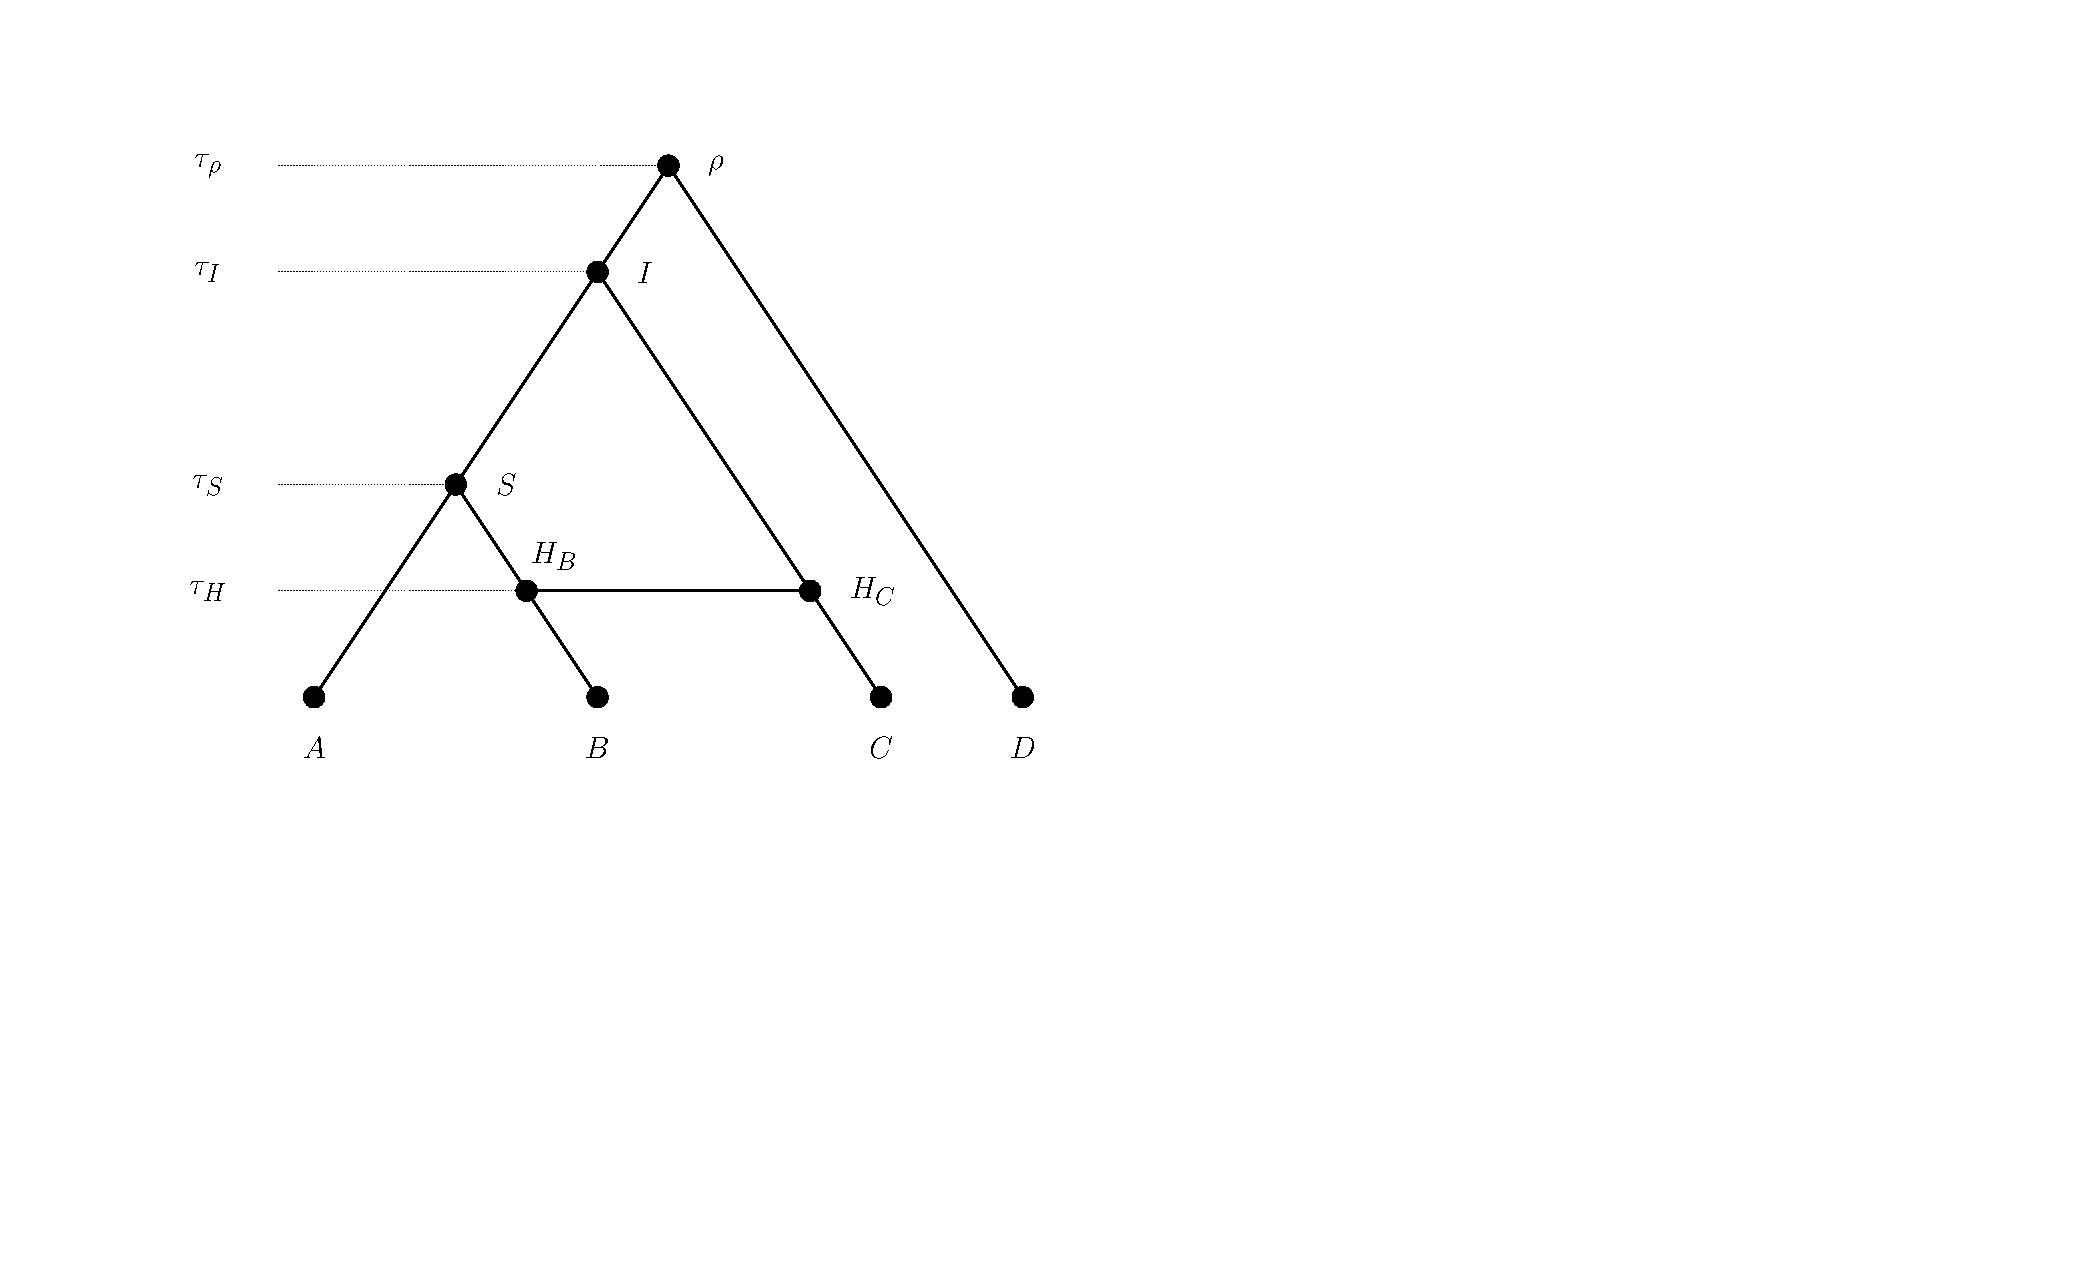
\includegraphics[scale=0.6]{figure1.pdf}
\scalebox{0.3}{\begin{tikzpicture}[font=\Huge]
\coordinate  (root) at (11,16);
\coordinate [label=right:$\rho$] (rootlabel) at (12,16);
\coordinate (tipa) at (1,1);
\coordinate [label=below:$A$] (alabel) at (1,0);
\coordinate (tipb) at (9,1);
\coordinate [label=below:$B$] (blabel) at (9,0);
\coordinate (tipc) at (17,1);
\coordinate [label=below:$C$] (clabel) at (17,0);
\coordinate (tipd) at (21,1);
\coordinate [label=below:$D$] (dlabel) at (21,0);
\coordinate (sisters) at (5,7);
\coordinate [label=right:$S$] (slabel) at (6,7);
\coordinate (ingroup) at (9,13);
\coordinate [label=right:$I$] (ilabel) at (10,13);
\coordinate (hybsis) at (7,4);
\coordinate [label=right:$H_B$] (hblabel) at (7,5);
\coordinate (hybouter) at (15,4);
\coordinate [label=right:$H_C$] (hclabel) at (16,4);
\fill (root) circle (2ex);
\fill (tipa) circle (2ex);
\fill (tipb) circle (2ex);
\fill (tipc) circle (2ex);
\fill (tipd) circle (2ex);
\draw[ultra thick] [-] (root) -- (tipa) ;
\draw[ultra thick] [-] (root) -- (tipd);
\fill (sisters) circle (2ex);
\fill (ingroup) circle (2ex);
\draw[ultra thick] [-] (sisters) -- (tipb);
\draw[ultra thick] [-] (ingroup) -- (tipc);
\fill (hybsis) circle (2ex);
\fill (hybouter) circle (2ex);
\draw[ultra thick] [-] (hybsis) -- (hybouter);
\draw[dotted] [-] (0,4) -- (7,4);
\node[] at (-2,4) {$\tau_H$};
\draw[dotted] [-] (0,7) -- (5,7);
\node[] at (-2,7) {$\tau_S$};
\draw[dotted] [-] (0,13) -- (9,13);
\node[] at (-2,13) {$\tau_I$};
\draw[dotted] [-] (0,16) -- (11,16);
\node[] at (-2,16) {$\tau_\rho$};
\end{tikzpicture}

}
\caption{The tree with node labelings and  the node depth parameters used throughout these notes. We consider a rooted four-taxon tree with a single outgroup ($D$) and hybridization/introgression event between two non-sister taxa ($B$ and $C$) in the ingroup. The hybridization/introgression nodes are labeled with $H$ and with a $B$ or $C$ subscript indicating which tip they are a parent to. The internal tree-nodes are labelled $S$, $I$, and $\eta$ to denote the sister, ingroup and root, respectively.}
\label{fig:tree}
\end{figure}

\subsection{Algorithm}
\subsubsection{Overview}
Most of the calculations are the same as in PoMo.
To deal with the hybridization/introgression event, we introduce a partial likelihood arrays (PLA) immediately before and after the event; in other words rootward and tipward of $H_B$ and $H_C$.
We will use $\uparrow$ to denote the rootward side of a node and $\downarrow$ to denote the tipward side of a node.
The only transitions between the two are the result of the mixing (with probability $\phi$ and weighting $\gamma_B$ and $\gamma_C$).


The rootward PLA has the size that is the square of the PoMo state space, because we need to account for the joint events: the probability that the $H_{B\uparrow}$ is in state $i$ and $H_{C\uparrow}$ is in state $j$ in order to correctly calculate the probability of the data tipward of the hybridization/introgression event.
But this expanded state space only affects a few nodes (because our tree is small, and we re-condense to the PoMo state space at node $I$.

\subsubsection{Notation}
We will use the notation of \cite{borges2020consistency} as much as possible.

Because all sites follow the same model the calculations described would be calculated for each data pattern.
Here we will elide the introduction of a dimension and indexing to refer to each data pattern, but in a real implementation the data structures would be arrays of the ones described below with an index for the site pattern.

The data consists of a vector of the four observed counts of each of the nucleotides for each of the four tips. 
We'll use 0=A, 1=C, 2=G, and 3=T to encode the nucleotides. So $C_A$, $C_B$, $C_C$, and $C_D$ would be vectors of for integers for the number of times each base was observed in that taxon in our sample from that species.
So $C_A[0]$ would hold the number of gene copies from population $A$ that were scored as having adenine.
Note that if we just have genotypic calls then a homozygous AA call would contribute 2 to this count, while a heterozygote such as AG would contribute 1.



PoMo models do not allow more than 2 nucleotides to be present in a population. So, any site having more than 2 non-zero counts would have a likelihood of zero and must be excluded (or not used with this model).
We'll use $O(C_A)$ to mean the set of nucleotides observed with counts greater than 1 in $A$.




We are considering nucleotide data so $K=4$.
Let $N$ be the the PoMo population size, typically a small number -- often 10 in prior work, but we will probably use only 4 for computational reasons.
If $\mathbb{A}$ denotes the set of all PoMo states, the number of PoMo states is $$|\mathbb{A}| = K + (N-1) {K \choose 2} $$
so in the nucleotide case:
$$|\mathbb{A}| = 4 + 6(N-1)$$
As in \cite{borges2020consistency}, we will denote the PoMo states as $\{N a_i \}$ to the state means monomorphic for allele $i$.
We will use $\{n_k a_i, (N-n_k) a_j \}$  to denote polymorphic containing $n_k$ copies of allele $i$ and $(N-n_k)$ copies of allele $j$, where $a_i$ and $a_j$ are denote nucleotides in the set $\{0,1,2,3\}$.

We will use $G_x$ to denote a partial likelihood vector or multi-dimensional array storing probabilities of events associated with node $x$. Later $G_x$ and $F_x$ will be used other partial likelihood structures to ease notation.

\subsubsection{Leaf Partial Likelihood Structures}
So, as in the standard PoMo approach,
$G_A[\alpha]$ will hold the probability of observing the nucleotide data, $C_A$, if the PoMo state were at node $A$ (denoted $p_A$) is $\alpha$:
$$G_A[\alpha] = \Pr\left(C_A\mid p_A = \alpha, \theta\right).$$

This can be calculated via:
\begin{equation}
G_A[\alpha=\{N a_i \}] = \left\{
  \begin{array}{ll}
    1 & \mbox{if } O(C_A) = \{a_i\} \\
    0 & \mbox{otherwise.} \\
  \end{array}\right.
\end{equation}
and
\begin{equation}
G_A[\alpha=\{n_k a_i, (N-n_k) a_j \}] = \left\{
  \begin{array}{ll}
  0 & \mbox{if } O(C_A) \neq \{a_i, a_j\} \\
    \left(\frac{n}{N}\right)^{C_A[a_i]}\left(\frac{N-n}{N}\right)^{C_A[a_j]} & \mbox{otherwise.}  
  \end{array}\right. 
\end{equation}
The same logic would be used to fill $G_B$, $G_C$ and $G_D$, based on the data  in $C_B$, $C_C$, and $C_D$ respectively.
\subsubsection{Post-hybridization/introgression Partial Likelihood Structures}
$G_{HB\downarrow}[\alpha]$ and $G_{HC\downarrow}[\alpha]$ hold the probability of observing the data at the tips $B$ and $C$ respectively if the PoMo process were in state $\alpha$ at time point $\tau_{H}$ and 
no further hybridization/introgression occurred:
$$G_{HB\downarrow}[\alpha] = \Pr\left(C_B\mid p_{HB\downarrow}=\alpha, \theta, \tau_H\right)$$
and
$$G_{HC\downarrow}[\alpha] = \Pr\left(C_C\mid p_{HC\downarrow}=\alpha, \theta, \tau_H\right).$$

This is a normal phylogenetic calculation:
\begin{equation}
G_{HB\downarrow}[i] = \sum_{j\in \mathbb{A}} G_B[j]\Pr\left(i\rightarrow j \mid \theta, \tau_{H}\right)
\end{equation}
where  $\theta$ denotes the numerical parameters of the PoMo model, and the $\Pr(\ldots)$ expression is the transition probability obtained by considering that PoMo process along a branch of length $\tau_{H}$.

$G_{HC\downarrow}$ is calculated in the same manner, except that $G_C$ is used as the leaf partial likelihood structure.

\subsubsection{Pre-hybridization/introgression $G_{HB\uparrow}$ Partial Likelihood Structure}
$G_{HB\uparrow}[\alpha_i][\alpha_j]$ is a data structure that depends on the joint combination of states: $\alpha_i$ at $H_B$ immediately prior to hybridization/introgression and $\alpha_j$ at $H_C$ immediately prior to hybridization/introgression. 
It is a two-dimensional array with each dimension having $|\mathbb{A}|$ bins.

$$G_{HB\uparrow}[\alpha_i][\alpha_j] = \Pr\left(C_B, C_C\mid p_{HB\uparrow}=\alpha_i, p_{HC\uparrow}=\alpha_j, \phi, \gamma_B, \gamma_C, \theta, \tau_H\right)$$
and
$G_{HC\uparrow}$ is not used.


If we use a model in which $\phi = 1$ then all sites are affected by hybridization/introgression, but in the general case we may want to consider a chance that a site will not be affected by hybridization/introgression.
Thus:
\begin{equation}
G_{HB\uparrow}[\alpha_i][\alpha_j] = \phi G^{\dag}[\alpha_i][\alpha_j] + \left(1-\phi\right)G_{HB\downarrow}[\alpha_i]G_{HC\downarrow}[\alpha_j]
\end{equation}
Note that if a site is unaffected by hybridization/introgression, there is no opportunity for change of state in the instant leading along the branches to $B$ and $C$.
So, if $\phi=0$ then $G_{HB\uparrow}[\alpha_i][\alpha_j]$ simply holds the product of the corresponding partial likelihood structures for the post-hybridization/introgression side of $H_B$ and $H_C$.

$G^{\dag}[\alpha_i][\alpha_j]$ holds the probability of observing the data at the leaves $B$ and $C$ conditional on the fact that the site was affected by hybridization/introgression at $\tau_{H}$.
If we allow for asymmetric hybridization/introgression and mixing frequencies $\neq 0.5$ (rather than complete apomixis at affected sites), then we can say:
\begin{equation}
G^{\dag}[\alpha_i][\alpha_j] = \left(\sum_{k\in \mathbb{A}}F_B[\alpha_i][\alpha_j][k]\right)
                        \left(\sum_{k\in \mathbb{A}}F_C[\alpha_i][\alpha_j][k]\right)
\end{equation}
where $F_B$ and $F_C$ are partial likelihood structures:
\begin{equation}
F_B[\alpha_i][\alpha_j][k] = \Pr\left(\alpha^{\dag}=k | \gamma_B, \alpha_i, \alpha_j\right)G_{B\downarrow}[k]
\end{equation}
where $\alpha^{\dag}$ denotes a PoMo state after the event.
$F_B[\alpha_i][\alpha_j][k]$ thus represents the probability of explaining the data for tip $B$ conditional on the pre-hybridization/introgression PoMo states being $\alpha_i$ for node $H_B$ and $\alpha_j$ for node $H_C$ and the post-hybridization/introgression PoMo state for node $H_B$ being $k$.



While the size of $F_B$ and $F_C$ appear to be $|\mathbb{A}|^3$, here we explore a hybridization/introgression transition probability function that assigns 0 probability to many of the post-hybridization/introgression PoMo.
Thus, we need not fill in the entirety of the third dimension (indexed by $k$ above) of these data structures.

We will refer to $\Pr\left(\alpha^{\dag}=k | \gamma, \alpha_i, \alpha_j\right)$ for any PoMo states as the hybridization/introgression transition probability mass function.
An appealing way to model hybridization/introgression would be for the allele frequencies to be simply the
weighted average of the pre-hybridization/introgression lineages' frequencies, where the introgressing lineage
is given a weight $\gamma$ and the lineage receiving the immigrants is given weight $(1-\gamma)$.
If $f()$ is used to denote the allele frequency vector for a PoMo state, and $f^{\dag}_B$ as the post-hybridization/introgression allele frequency in the space of a 4-dimensional simplex, we could say:
\begin{equation}
f^{\dag}_B = \left(1-\gamma_B\right) f(\alpha_i) + \gamma_B f(\alpha_j)
\end{equation}
However this weighted average approach would be a continuous trait that does not map to PoMo states (e.g. more than 2 alleles could have non-zero frequencies).
One could model the probabilities for the post-hybridization/introgression events using the probability mass function for multinomial for $N$ draws from $f^{\dag}_B$, conditional on the outcome being a PoMo state.

A downside of an approach based on this multinomial is obvious when we consider $\gamma_B=0$.
In that case, species  at $H_B$ does not get any immigration from $H_C$, thus the hybridization/introgression event should have no affect on the PoMo state along lineage $B$.
In such case, we should prefer the hybridization/introgression event to have no effect on the evolution of lineage $B$, so for the instantaneous hybridization/introgression event $\Pr\left(\alpha^{\dag}=k | \gamma_B=1, \alpha_i, \alpha_j\right)= 1$ if $k=i$ and 0 otherwise.
However, if the lineage $B$ were in the PoMo state $\{2a_i, 2a_j\}$, a multinomial draw would assign some probability to an instantaneous transition to $\{4a_i\}$ and to $\{4a_j\}$.
This could result in the introduction of hybridization/introgression events with $\gamma_0$ as way of explaining faster than expected drift rather than hybridization/introgression.

Similarly if $H_B$ and $H_C$ both have the same (polymorphic) PoMo state, then hybridization/introgression should
have no effect, but a multinomial-based approach would for an instantaneous jump in allele frequencies
at the hybridization/introgression event.

To avoid this we can consider a simple set of rules of modeling the change in PoMo states such that probability mass is put only a few PoMo states.
First we would like the PoMo transitional probability to be independent of $\gamma_B$, $\alpha_i$, and $\alpha_j$, conditional on $f^{\dag}_B$:
\begin{equation}
    \Pr\left(\alpha^{\dag}=k |f^{\dag}_B, \gamma, \alpha_i, \alpha_j\right) = \Pr\left(\alpha^{\dag}=k | f^{\dag}_B\right)
\end{equation}

The first rule is that:
\begin{equation}
    \Pr\left(\alpha^{\dag}=k | f^{\dag}_B\right)=1\mbox{ if }f(k) = f^{\dag}_B
\end{equation}
This guarantees that hybridization/introgression does not change the PoMo states in the cases mentioned above ($\gamma_B=0$ or same PoMo states in $H_B$ and $H_C$ before hybridization/introgression)

Let $d()$ be a distance function (we'll use the Euclidean distance, initially) for the distance between two probability vectors.

If $f(k) \neq f^{\dag}_B$ for any PoMo state $k$, then we calculate $d(f(k), f^{\dag}_B)$ for every PoMo state.
let $Q$ be the set of states that are tied for being closest to $f^{\dag}_B$, and $R$ be the set of states that are tied for being second-closest to $f^{\dag}_B$.

If $|Q| > 1$ then
\begin{equation}
    \Pr\left(\alpha^{\dag}=k | f^{\dag}_B\right)= \left\{
  \begin{array}{ll}
   0 & \forall k \notin Q  \\
   1/|Q| & \forall k \in Q  \\
   \end{array}\right.
\end{equation}

If $|Q| = 1$ and $|R| = 1$ then, we will denote the PoMo states in these sets as $q$ and $r$. respectively.
Let $d_T = d\left(f(q), f^{\dag}_B\right) +  d\left(f(r), f^{\dag}_B\right)$. Then:
\begin{equation}
    \Pr\left(\alpha^{\dag}=k | f^{\dag}_B\right)= \left\{
  \begin{array}{ll}
   0 & \forall k \notin Q \mbox{ and }  k \notin R \\
   d(f(r),f^{\dag}_B)/d_T  & \mbox{if } k=q  \\
   d(f(q),f^{\dag}_B)/d_T & \mbox{if } k=r \\
   \end{array}\right.
\end{equation}
In words the probability of going to the closest state is proportional to the ``closeness'' to that state in the sense of the fraction of the total distance is contributed by the second-closest state.
So as the distances  to the closest and second closest states get closer to each other, the probability mass function gets closer to the case in which states $q$ and $r$ are tied for being the closest.
Similarly as $f^{\dag}_B$ gets closer and closer to $f(q)$, the probability associated with that state approaches 1.

The final case is if $|Q| = 1$ and $|R| > 1$. 
Now we let $q$ denote the member of $Q$ and $r$ denote any member of $R$.
Let $m=d(f(r),f^{\dag}_B)/d(f(q),f^{\dag}_B)$ then:
\begin{equation}
    \Pr\left(\alpha^{\dag}=k | f^{\dag}_B\right)= \left\{
  \begin{array}{ll}
   0 & \forall k \notin Q \mbox{ and }  k \notin R \\
   m/(m+|R|)  & \mbox{if } k=q  \\
   1/(m+|R|) & \mbox{if } k\in R \\
   \end{array}\right.
\end{equation}

The approach taken for filling $F_C$ is the same as for $F_B$.
$F_C$ in it  we uses $G_{C\downarrow}$ rather than $G_{B\downarrow}$ and
\begin{equation}
f^{\dag}_C = \left(1-\gamma_C\right) f(\alpha_j) + \gamma_C f(\alpha_i)
\end{equation}
is used for calculating the hybridization/introgression transition probability function.

\subsubsection{The sister node $G_S$ Partial Likelihood Structure}
The calculations involved in partial likelihoods at the sister node $S$, are standard internal node PoMo calculations, however there is extra bookkeeping because on descendant partial likelihood structure, $G_A$, has
the standard dimensionality of 1 with the number of PoMo states, while the other ($G_{HB\uparrow}[i][j]$) is a two-dimensional matrix of size $|\mathbb{A}|\times |\mathbb{A}|$.
So:
$$G_{S}[\alpha_i][\alpha_j] = \Pr\left(C_A, C_B, C_C\mid p_S=\alpha_i, p_{HC\uparrow}=\alpha_j, \phi, \gamma_B, \gamma_C, \theta, \tau_H, \tau_S\right).$$

The second dimension of the $G_{HB\uparrow}[i][j]$ indexes the state pre-hybridization/introgression at $H_C$.
Because the evolution from $I\rightarrow H_C$ is independent of the evolution from $S\rightarrow H_B$ 
and $S\rightarrow A$, the calculations do not change from the normal phylogenetic calculation:
\begin{equation}
G_{S}[\alpha=i][j] = \left[\sum_{k\in \mathbb{A}} G_{HB\uparrow}[k][j]\Pr\left(i\rightarrow k \mid \theta, \tau_S - \tau_{H}\right)\right]
\left[\sum_{k\in \mathbb{A}} G_{A}[k]\Pr\left(i\rightarrow k \mid \theta, \tau_S \right)\right]
\end{equation}
Note that the state at $H_C$ (indexed by $j$) does not occur in the right summation, so that results of that summation could be stored in a vector of size $|\mathbb{A}|$ rather than conducting the summation multiple times.

\subsubsection{The ingroup node $G_I$ Partial Likelihood Structure}
As in $G_S$, the approach is the standard PoMo calculation with extra indexing for the branch from $I\rightarrow S$, on the branch from $I\rightarrow H_C$ we just need to calculate the probability that a PoMo state at $I$ would yield a PoMo state at $H_C$ because the $G_{S}[\alpha=i][j]$ holds the probability of the data in $C_A$, $C_B$, and $C_C$ {\em conditional} on state $j$ at $H_C$.
$$G_{I}[\alpha_i]= \Pr\left(C_A, C_B, C_C\mid p_I=\alpha_i, \phi, \gamma_B, \gamma_C, \theta, \tau_H, \tau_S, \tau_I\right).$$


At $I$ we can collapse back down to a data structure that is a vector of length $|\mathbb{A}$:
\begin{equation}
G_{I}[\alpha=i] = \sum_{j\in \mathbb{A}}\Pr\left(i\rightarrow j \mid \theta, \tau_S - \tau_H \right)
 \left[\sum_{k\in \mathbb{A}} G_{S}[k][j]\Pr\left(i\rightarrow k \mid \theta, \tau_I - \tau_{S}\right)\right]
\end{equation}

\subsubsection{The root node $G_\eta$ Partial Likelihood Structure and Likelihood}
At the root, it is simply standard PoMo:
\begin{equation}
G_{\eta}[\alpha=i] = \left[\sum_{k\in \mathbb{A}} G_{I}[k]\Pr\left(i\rightarrow k \mid \theta, \tau_{\eta} - \tau_{I}\right)\right]\left[\sum_{k\in \mathbb{A}} G_{D}[k]\Pr\left(i\rightarrow k \mid \theta, \tau_{\eta} \right)\right]
\end{equation}
and 
$$G_{\eta}[\alpha_i]= \Pr\left(C_A, C_B, C_C, C_D\mid p_{\eta}=\alpha_i, \phi, \gamma_B, \gamma_C, \theta, \tau_H, \tau_S, \tau_I, \tau_{\eta}\right).$$

Thus, the likelihood is:
\begin{equation}
\Pr\left(C_A,C_B,C_C, C_D\mid \phi, \gamma_B, \gamma_C, \theta, \tau_H, \tau_S, \tau_I, \tau_{\eta}\right)  = \sum_{i\in \mathbb{A}} {\bm \psi}[i] G_{\eta}[\alpha=i]
\end{equation}
where ${\bm \psi}[i]$ is the stationary frequency of PoMo state $i$ as derived in \cite{BorgesSK2019}:
\begin{equation}
{\bm \psi}[x] = \left\{
  \begin{array}{rl}
    \frac{\pi_{a_i} \left(1 + \sigma_{a_i}\right)^{N-1}}{k}& \mbox{if } x=\{Na_i\} \\
    & \\
    \frac{N\pi_{a_i}\pi_{a_j}\rho_{a_i a_j} \left(1 + \sigma_{a_i}\right)^{n-1}\left(1 + \sigma_{a_j}\right)^{N-n-1}}{n(N-n)k} & \mbox{if }x=\{na_i, (N-n)a_j\} \\
  \end{array}\right.\label{stationary}
\end{equation}
where $\pi_{a_i}$ is the nucleotide frequency of base $a_i$, $\sigma_{a_i}$ is the relative selective coefficient of base $a_i$ (which is 0 for all bases if we are considering the neutral case), $\rho_{a_i a_j}$ is the nucleotide exchangeability parameter for a $a_i\rightarrow a_j$ mutation, and $k$
is the normalizing constant.
$k$ is calculated by simply summing all of the unnormalized stationary frequencies ({\em i.e.} set $k=1$, then sum all the possible forms of Eqn \ref{stationary} to arrive at the true value of $k$). 

For the neutral case:
\begin{equation}
{\bm \psi}[x] = \left\{
  \begin{array}{rl}
    \frac{\pi_{a_i} }{k}& \mbox{if } x=\{Na_i\} \\
    & \\
    \frac{N\pi_{a_i}\pi_{a_j} \rho_{a_i a_j}}{n(N-n)k} & \mbox{if }x=\{na_i, (N-n)a_j\} \\
  \end{array}\right.\label{stationaryneutral}
\end{equation}



\section{TODO}
\begin{enumerate}
    \item Implement the calculations in either Bayesian or ML context
    \item Simulate data sets with and without hybridization/introgression and see if the software implementation prefers the true model
    \item analyze Lucas' and Devon's data with the model
    \item Publish and await Nobel Prize
\end{enumerate}

\bibliographystyle{apacite}
\bibliography{pomorefs}


\end{document}
%F_B[\{n_k a_i, (N-n_k) a_j \}][\alpha_j] = {N\choose n_k}


